\documentclass[a4paper]{article}

\input{~/templates/math.tex}
\newtheorem{question}{Question}
\usepackage{fullpage}
\usepackage{exercise}
\newtheorem{exercise}{Exercise}[section]
% \usepackage{yhmath}
\DeclareMathOperator{\Sym}{Sym_1}

\title{Arithmetic Combinatorics}
\author{Vincent Tran}

\begin{document}
\maketitle

\section{3/19 - Elementary Methods}

\subsection{Inverse Theorems}

We will look at sum sets, product sets, and a few times quotient sets.

The context for this will be $G $, an abelian group. We are interested in $\Z, \Z^d, \R^d, \Z_p \coloneqq \Z / p\Z, \Z_2^n$. Let $A,B,C $ be finite subsets of $G $. In addition, all sets will be non-empty.

\begin{definition}
	\textbf{Minkowski Sum}
	\[
		A + B = \{a+b|a\in A, b\in B\}
	.\]
	\[
		A - B = \{a-b|a\in A, b\in B\}
	.\]

	Clearly $A+B $ is associative and commutative.

	Similarly,
	\[
		nA \coloneqq A + \cdots + A
	\]
	$n $ times.
\end{definition}

\begin{property}
	$nA - mA \ne (n-m)A $ in general, i.e. the Minkowski sum doesn't distribute.
\end{property}

\begin{question}
	When is $A+A $ small?
\end{question}

Trivially, we have
\[
	|A| \le |A+A| \le |A|^2
.\]

We are looking for when $|A+A| $ is close to $|A| $.

Direct Problem: How small can $|A+A| $ be?

Inverse: For which $A $ is $|A+A| $ small?

\begin{example}
	Let $G = \Z $, $A = [0,n-1] $.
	Then $A+A = [0,2n-2] \implies |A+A| = 2|A|-1 $.

	By using affine transformations $\phi: \Z\to \Z $ defined by $\phi(x) = ax+b $, we have that $b, b+r, \ldots, b+(n-1)r $ is a value for $|A| $ s.t. $|A+A| = 2|A| -1 $.
\end{example}

\begin{definition}
	\textbf{Generalized Arithmetic Progressions}: They are of the form $b + r_{1}x_{1}+\cdots + r_dx_d $ where $x_i \in [0,n_i-1]$, i.e. affinely transformed sums of $A_i $.
\end{definition}

\begin{thm}
	$\forall A \subseteq \Z |A+A| \ge 2|A|-1$.
\end{thm}

\begin{proof}
	Proof 1: Induction. Let $A = \{a_{1} < a_{2} < \cdots < a_n\}   $ and define $A' = A \setminus \{a_n\}   $.
	By the induction hypothesis, $|A'+A'| \ge 2|A'| - 1 = 2n-3 $.
	By noticing that $2a_n, a_n + a_{n-1} $ are elements not in $A'+A' $ but are in $A+A $, we have that $|A+A| \ge 2|A| - 1 $.

	Proof 2: Go bi. We can generalize this theorem to more variables: $|A+B| \ge |A| + |B| - 1 $, in which case induction is ever simpler as only the largest element is needed.

	Proof 3: Take two sets $A,B $, represent them as cicles with elements in descending order in them.
	Take $|B| $ picks in $A $ and $|A| $ picks in $B $.
	Draw a bar connecting a pick in $A $ to a pick in $B $.
	Do this for all picks in $B $.
	Then do this for all picks in $A $ (above two steps).
	We then have found $|A| + |B| - 1 $ distinct elements (?).
\end{proof}

\begin{thm}[Cauchy-Davenport]
	For $G = \Z_p,\ |A+B| \ge \min(|A|+|B| - 1, p) $.
\end{thm}

\begin{definition}[\textbf{e-transform}]
	Fix an element $e \in A-B $.
	Then
	\begin{align*}
		A_{(e)} :\coloneqq  A \cup (B+e) \\
		B_{(e)} :\coloneqq B \cap (A - e)
	.\end{align*}
	See \Cref{fig:e-transform}
\end{definition}

\begin{figure}[ht]
	\centering
	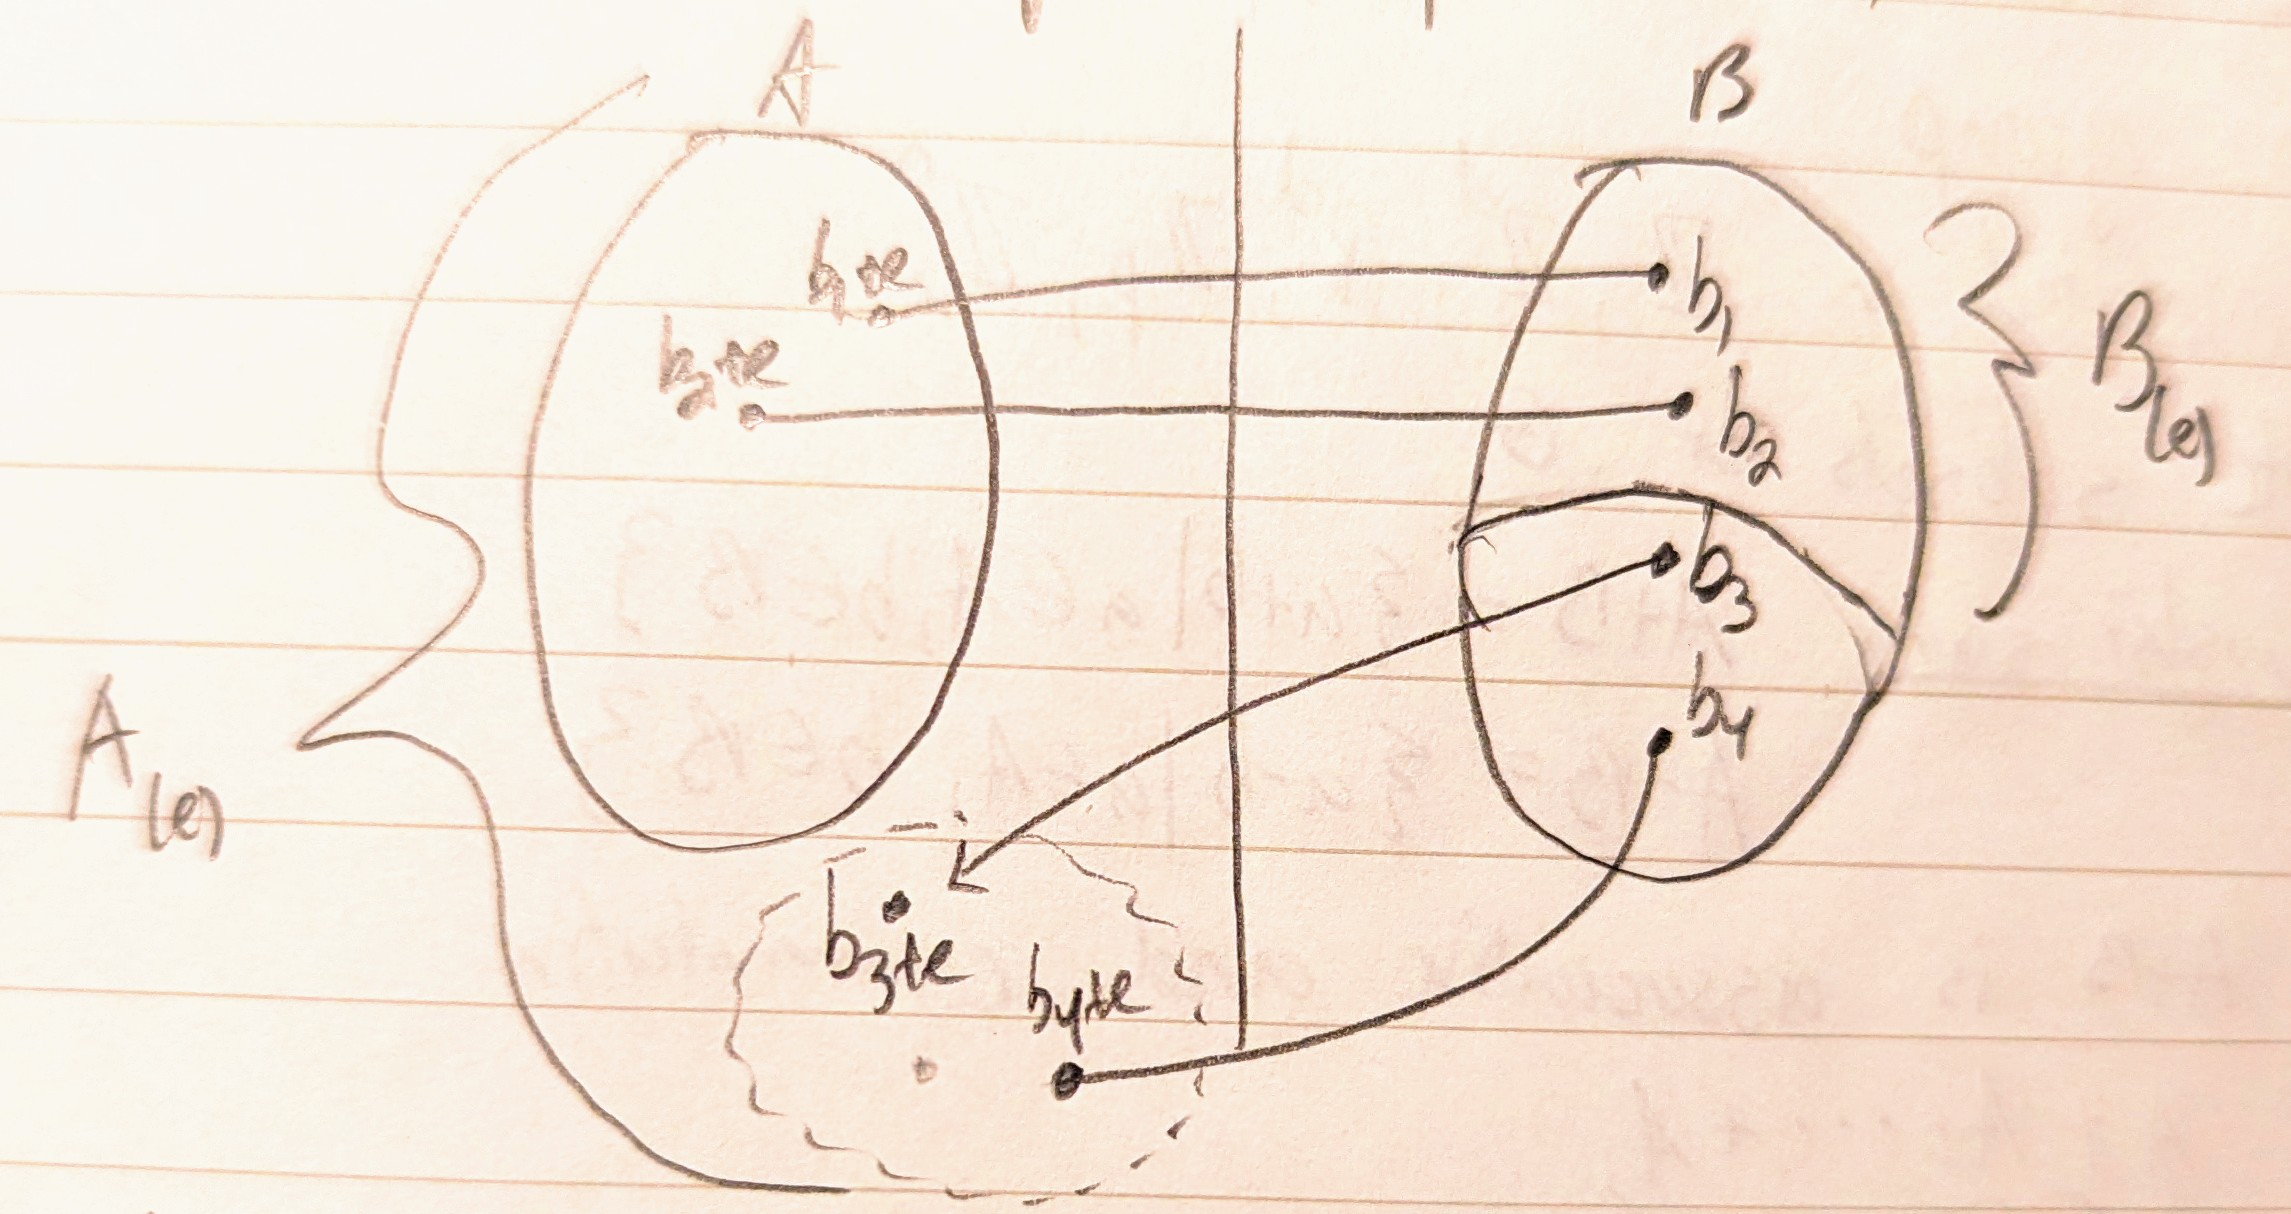
\includegraphics[width = .5\textwidth]{wall}
	\caption{The e-transform \label{fig:e-transform}}
\end{figure}

\begin{lem}
	\begin{enumerate}
		\item $|A_{(e)}| + |B_{(e)}| = |A| + |B| $
		\item $|A_{(e)}\ge |A| $
		\item $A_{(e)}+B_{(e)} \subseteq A+B $
	\end{enumerate}
\end{lem}
\begin{proof}
	For a), clearly $A_{(e)} $ contains $|A| $ elements plus some.
	Then for any element $b \in B $, $b+e \in A $ or $\not\in A $.

	If $b+e \in A $, then $b \in A-e \implies b \in B_{(e)} $.

	If $b+e \not\in A $, then obviously $b+e \in A_{(e)} $ and not in $A $.
	Thus $|A_{(e)}| + |B_{(e)}| = |A| + |B| $.

	b) is truly trivial.

	c) If we take $a \in A_{(e)} $ and it falls in $A $, then we are done as $B_{(e)} \subseteq B $.
	So the only hard case is when $a \in B+e \setminus A $.
	By definition, $A_{(e)}+B_{(e)} $ consists of $a + b, b \in B_{(e)} $ and hence $b \in A \setminus e $.
	Thus $b = a' - e \implies a + b = a + a'-e = b' + a'$ for $b' \in B $ since $a \in B+e $.
\end{proof}

\begin{proof}[Proof: Cauchy-Davenport]
	If $|B| = 1 $ then we are trivially done.
	We then use induction on the size of $B $ and the e-transform to see that $B_{(e)} = B \forall e \in A \setminus B $.
 	Hence $\forall e \in A- B,\ B+e \subseteq A \implies B + A-B \subseteq A $, i.e. $A + (B-B) \subseteq A $.

	As $|B| \ge 2 $, we can let $d = b_{1}-b_{2} $ and see that $A + d = A + (B-B) = A $ and the same is true for all multiples of $d $ (equality is true since $|A| \le |A+(B-B)| $).
	Since $A = \Z_p $ and we are done (this is the min).
\end{proof}

\begin{thm}[Vosper]
	For $A,B \subseteq \Z $ and $|A+B| = |A| + |B| - 1 $, then $A,B $ are a.p. (arithmetic progressions) with the same step.
\end{thm}
\begin{proof}
	(Proof from Tao, not class)

	First we handle three cases:

	$A $ or $B $ are arithmetic progressions: WLOG say $A $ is.
	Then $A = \{a, a + v, \ldots , a + nv\}   $.
	So then $|B| + n = |A| + |B| - 1 = |A+B|$ by hypothesis.

	WLOG let $A = \{a, a+v, \ldots , a + (n-1)v\}  + \{0,v\}   $ with $v $ positive.
	So $|A+B| = |\{a, \ldots, a + (n-1)v\}  + B + \{0,v\} | \ge n-1 + |B + \{0,v\} |$ by Cauchy-Davenport.
	By Cauchy-Davenport again, we have that $|B+\{0,v\} | \ge |B| + 1  $ and from above ($|B| + n \ge n-1 + |B+\{0,v\} |  $) we have that $|B| + 1 = |B + \{0,v\} |  $.

	The largest element of $B $ (say $b_n $) plus $v $ isn't in $B $, so this is the only element of $B + \{0,v\}$ that isn't in $B $, giving us that $B \setminus \{b_n\} + v \subseteq B$.
	Hence $B $ is an arithmetic progression.

	If $|A+B| $ is an arithmetic progression, then let $C = -(\Z_p \setminus (A+B)) $.
	Notice that $|C| = p - |A+B| = p + 1 - |A| - |B|$.
	It follows that $C $ is an arithmetic progression with the same step because the step is an additive generator in $\Z_p $.
	As such if we continue out the progression and reversed it (by negating), we would get the later half that isn't in $-(A+B) $.

	Next we can see that $C+B \subseteq (\Z_p \setminus A)$ because if $C+B $ intersected $-A $ at say $-a = c+b $, then $-(a + b)$ would be in $-(A+B) $ but also $C $, a contradiction.
	Hence $p - |A| \ge |C+B| \ge |C|+|B| - 1 = p - |A|$ by Cauchy-Davenport.
	So $|C+B| = p - |A| = |C| + |B| - 1$.
	By the work before, this gives us that $B $ is an arithmetic progression of the same step as $C $.
	Similarly for $A $.

	Now to prove this for when none of them are arithmetic progressions.
	We use induction.
	For $|B| = 2 $, we have that $B $ is an arithmetic progression and we are done.

	$|B| > 2 $:
	We have two cases:

	$1 < |B_{(e)}| < |B|$ for some $e \in A-B $:
	By the lemma and starting hypothesis, $|A_{(e)}+B_{(e)}| = |A_{(e)}| + |B_{(e)}| - 1 $ and by the inductive hypothesis $B_{(e)} $ and $A_{(e)} $ are arithmetic progressions with the same step.
	Hence $A+B = A_{(e)} + B_{(e)}$ is an arithmetic progression, reducing us back into the previous case.

	$|B_{(e)}| = |B|$ or 1 $\forall e \in A-B$.
	Let $E \subseteq A - B$ be the set of $e $ s.t. $|B_{(e)}| = |B| $.
	Then $B + E \subseteq A $ and by Cauchy-Davenport, we have that $|B| + |E| - 1 \le |A| \iff |E| \le |A| - |B| + 1 $.
	Since $|A - B| \ge |A| + |B| - 1 $ by Cauchy-Davenport, by pidgeonhole principle there are at least $2|B| - 2$ values of $e $.
	By pidgeonhole again, we have $e,e' $ s.t. $B_{(e)} = B_{(e')} = \{b\} $.

	Since $|A+B| = |A| + |B| - 1 $, $A+B = A_{(e)} + b = A_{(e')} + b $ and thus $A\cup (B+e) = A \cup (B+e') $.
	As $|B_{(e)}| = 1 $, $A \cap B+e = b + e$ and similarly for $e' $, $B+e $ and $B+e' $ differ by at most one element (use the fact that $A\cup (B+e) = A \cup (B+e')$).
	Hence $B $ is an arithmetic sequence of $e' - e $.
\end{proof}

\section{3/21/24}

Let $A \subseteq G $ be non-empty and finite.

\begin{definition}
	\textbf{$\Sym(A) $} $\coloneqq \{x | x+A = A\}   $.
	This is clearly a subgroup of $G $.
\end{definition}

\begin{thm}[Kneser (53)]
	Let $A,B \subseteq G, G = \Sym(A+B) $.
	Then $|A+B| \ge |A+H| + |B+H| - |H| $.
\end{thm}

\begin{proof}
	Proof 1: Induction on 4 parameters.

	Proof 2:
	For $\Z $, $|H| = 1 $ because $H $ has to be 0 by ordering $A $.
	Then the statement is $|A+B| \ge |A| + |B| - 1 $, done by Cauchy-Davenport.

	For $\Z_p $, $H= 0 $ or $\Z_p $ as the only subgroups of $\Z_p $.
	This is trivial.
\end{proof}

At this point, we know a lot about when $|A| = n, |A+A| = 2n-1$ (by Vosper's), and now we can get information about $|A+A| = 2n-1 + b, b \le n-1$:

\begin{thm}[Freiman's $3k-3 $]
	For $A\subseteq \Z $ and $|A+A| = 2n-1 + b $ for $b \le n-1 $, then $A $ is a subset of an $n+b $ term arithmetic progression.
\end{thm}

\begin{example}
	We can generate examples by letting $A = \{0,\ldots ,n-2, n-1+b\} \subset \{0,1,\ldots ,n+b\}    $.
	Notice that $|A+A| = 2n+b-1 $ because of three cases:
	\[
		\begin{cases}
			[0,n-2] + [0,n-2] = [0,2n-2]\\
			[0,n-2] + \{n-1+b\}  = [2n-2,2n-2+b]\\
			\{n-1+b\} + \{n-1+b\}  = \{2n-2+2b\}
		\end{cases}
	.\]
	This is $2n-1+b $ elements.
\end{example}

\subsection{Digression into Some Combinatorics}

This is a treasured result in combinatorics, and will use a similar technique as the e-transform.

\begin{definition}
	$[n] \coloneqq \{1,\ldots,n\}   $.
\end{definition}

\begin{definition}
	$\Delta\subseteq \mathcal{P}([n]) $ is an \textbf{ideal} if $\forall F\in \Delta , G\subseteq F \implies G \in \Delta$.
\end{definition}

\begin{definition}
	\[
		\binom{[n]}{k} \coloneqq  \{F\subseteq [n] \vert |F| = k\}
	.\]
\end{definition}

\begin{definition}
	The \textbf{shadow} of $\mathcal{F} = \Delta \cap \binom{[n]}{k}$ to be $\partial \mathcal{F} \coloneqq \{G \in \binom{[n]}{k} | \exists F \in \mathcal{F}, |F \setminus G| = 1\}   $.
	Intuitively, the shadow compacts sets, much like the e-transform.
\end{definition}

\begin{thm}[Kruskal-Katoma]
	Let $|\mathcal{F}| = m $ and find $x $ s.t. $m = \binom{x}{k} $.
	Then
	\[
		|\partial \mathcal{F}| \ge \binom{x}{k-1}
	.\]
\end{thm}

An equivalent statement is that given $\{i_{1} < i_{2} < \cdots < i_k \} \in \binom{[n]}{k}  $, we can view it as the string $[i_k,\ldots,i_{1}] $ and order the $\binom{[n]}{k} $ lexicographically.
Then let $\mathcal{R}(m,k) $ be the $m $ smallest elements in this ordering.
The equivalent statement is that $|\partial(\mathcal{F})| \ge |\partial(\mathcal{R}(m,k))| $.

\begin{definition}
	\begin{align*}
		S_{ij}: \mathcal{P}([n]) &\longrightarrow  \mathcal{P}([n])\\
		S_{ij}(A) &=
		\begin{cases}
			A \setminus \{j\} \cup \{i\}  & \text{ if $j \in A $ and $i \not\in A $}\\
			A & \text{ else}
		\end{cases}
	.\end{align*}

	\begin{align*}
		S_{ij}: \mathcal{P}(\mathcal{P}([n])) &\longrightarrow \mathcal{P}(\mathcal{P}([n]))\\
		S_{ij}(\mathcal{H}) \coloneqq \{S_{ij}(H), \forall i,j\}
	.\end{align*}

	Intuitively, this is trying to get $G $ through the ``wall'' using $S_{ij} $.
	This is analogous to the e-transform from before.
\end{definition}

\begin{lem}
	For $\mathcal{F} \subseteq \binom{[n]}{k} $ and $\partial(S_{ij}(\mathcal{F})) \subseteq S_{ij}(\partial \mathcal{F}) $, then $|\partial (S_{ij}\mathcal{F})| \le |S_{ij}(\partial(\mathcal{F}))|$.
\end{lem}

\begin{proof}
	For $G \in \partial(S_{ij}(\mathcal{F}))$, we have that $G + \ell \in S_{ij}(\mathcal{F}) $ for some $\ell $.
	If this is true up to $k-1 $, then when $G \cup i \setminus j \in \partial(\mathcal{F}) $, then .we can just swap $i,j $ and find that $G \in S_{ij}(\partial \mathcal{F}) $.
	Let $G' $ be a preimage of $G + \ell $.

	Case one is that $G' + \ell\in \mathcal{F} $.
	% $G'\cup \ell \in \mathcal{F} $ ($G' $ being a difference set from $G \in \partial(S_{ij}(\mathcal{F})) $).
	The only case is $G \cup i \setminus j \not\in \partial (\mathcal{F}) $.
	If $i = \ell $, then $G' \cup \ell -j \in \partial(\mathcal{F}) $, a contradiction.

	If $i \ne \ell$: $G' \cup i \not\in \mathcal{F} $ (otherwise $G' \in\partial \mathcal{F} $, completing the proof), which implies $G' \cup i \setminus j \setminus \ell \not\in \mathcal{F}$ because otherwise $G'\cup i \setminus j \in \partial(\mathcal{F})$ which completes it with a swap.
	But $G' + \ell\in \mathcal{F} \implies $ we can shift and have $G \cup \ell=G' \setminus j \cup i \cup \ell \in S_{ij}(\mathcal{F}) $.
	This then implies that $G \setminus j \cup i \in \partial(S_{ij}(F)) \implies G \in S_{ij}(\partial(S_{ij}(\mathcal{F}))) $.

	If $G' \cup \ell\not\in \mathcal{F} $: Then $G \cup \ell \in S_{ij}(\mathcal{F}) \implies G \cup \ell \cup j \setminus i \in F $.
\end{proof}

\begin{proof}(Krushkal-Katoma)
	By the Lemma, we can assume no more shifts can be done.
	However, this doesn't trivialize the problem like the e-transform case: $\{\{1,2\} ,\{1,3\} ,\{1,4\}    \}   $ and $\{\{1,2\} ,\{2,3\} ,\{1,3\}    \}   $ are both extremal and we can't shift in.

	Define $\mathcal{F}(1) = \{F \vert 1 \in F\} , F(0) = \{F | 1 \not\in F\}    $.
	Assume this is true for smaller sets.
	We just need to show that $|\partial(F(0))| \le |F(1)|$.

	Take $G \in \partial(F(0)) $.
	Then $S_{e_{1}} $ doesn't affect $G $ by assumption, so $G \cup \{1\} \in F(1)	$ for an arbitrary element $e \in G $.
\end{proof}

\section{Doubling Constant}

\begin{definition}
	\[
	\delta[A] = \frac{|A+A|}{|A|}
	.\]
\end{definition}

We have dealt with $\delta[A] \le 2 $, the $3k-3 $ theorem gives us $\delta[A] \le 3 $.
In general, we need generalized arithmetic progressions.

This is Freiman's Theorem and the Polynomial Freiman-Rusza conjecture, which was solved recently in characteristic 2 by Gowers, Green, Manners, Tao.

How to construct sets with small doubling constants?

For $A $ an arithmetic progression, we are done.
Define $A,B $ as independent if $|A+B| = |A|\cdot |B|$.
Then
\[
	\delta[A+B] = \frac{|A+B+A+B|}{|A+B|} = \frac{|(A+A)+(B+B)|}{|A|\cdot|B|} \le \frac{|A+A|}{|A|} \cdot \frac{|B+B|}{|B|} \le \delta[A] \cdot \delta[B]
.\]

\section{3/26/24}

Now we look to generalized arithmetic progressions (gap) of rank $d $: $A_{1} + \cdots + A_d $ with $A_i $ being ap.

\begin{definition}
	A gap is \textbf{proper} if $|A_{1}+\cdots+A_d| = |A_{1}|\cdot|A_{2}|\cdots |A_d| $
\end{definition}

$P $ is a proper ap $\implies \delta[P] \le 2^d $ with $d = \rank(P) $.

Now suppose $B\subseteq A $ and let $\mu = \frac{|B|}{|A|} $.
Then $\delta[B] = \frac{|B+B|}{|B|} \le \frac{|A+A|}{|B|} = \mu ^{-1}\delta[A] $.

There are two cases for the group:
\begin{itemize}
	\item Torsion Free (e.g. $\Z,\Z_p^d,\R^d $)
	\item Forsion (e.g. $\Z_2^n $)
\end{itemize}

\begin{thm}[Freiman (Torsion Free)]
	Fix an integer $k $.
	Then $\exists $ constants $d,\mu $ (depending on $k $ only) s.t. $\forall A\subseteq \Z $ and $\delta[A] = k $, then there exists a propery gap $P $ s.t. $\rank(P)\le d $, $A \subseteq P $, and $\frac{|P|}{|A|}\le \mu ^{-1} $.
\end{thm}

\begin{cor}
	$\delta[A] \le \mu ^{-1}2^d $
\end{cor}

The point of this is that $\exists \mu ^{-1}, d \le k^{o(1)}  $.

We really want $d $ to be tight to $k $.

But we can always find a crazy set $|X| = k $ and $\delta[X] = k $ s.t. $d$ has to be $k $.

\begin{conj}[Polynomial Freiman-Rusza Conjecture]
	For $A\subseteq P + X $ with $|X| \le k^{O(1)}$, $\rank(A) \le O(\log K) $.
\end{conj}

\begin{thm}[Gowers, Green, Manners, Tao (23)]
	$\forall A \subseteq \Z_2^n $ with $\delta[A] =k $, $\exists H \subseteq \Z_2^n $ s.t. $\exists X(|X| \le k^{O(1)})  $ s.t. $A\subseteq H + X $, then $|H| \le k^{O(1)}|A|  $.
\end{thm}

Some History:

\begin{enumerate}
	\item Freiman's Proof (didn't draw much attention)
	\item Rusza's Proof which brought in analysis $\rightarrow $ more attention
	\item Sanders proved quasi-polynomial Freiman Rusza
	\item Recent GGMT polynomial FR conjection in characteristic 2 (promised in general as well)
\end{enumerate}

In this class 1, 2, and 4 will be discussed.

Let $A\subseteq \R^d $ (under addition). Freiman's can still apply here.

\begin{lem}[Freiman Dimension Reduction Lemma]
	Let $k = \delta[A], d=\operatorname{rk}(\operatorname{Span}(A))$.
	Then $|A+A| \ge (d+1)|A| - d(d+1) / 2 \implies \delta[A] \ge d+1, d \le k-1$.

	This is obviously false in $\char \ne 0 $.
\end{lem}

\begin{proof}
	We do induction on $|A| $.
	This is easily true for $|A| = 1. $

	Then for $|A| > 1 $, take the convex hull of $A $.
	Take a point $a\in A $.
	So $A' = A \setminus \{a\}  \implies |A' +A'| \ge (d'+1)|A'| - d'(d'+1) / 2$ by induction hypothesis.

	If $\operatorname{rk}(A') = d $, then $a \in A $ has $d $ neighbors, $a_{1},\ldots ,a_d $.
	The midpoints $\frac{a+a_{1}}{2},\ldots, \frac{a+a_d}{2} $ are not in $A' $ because otherwise $a \in A' $, a contradiction of the number of neighbors (?).
	Hence $a+a_{1},\ldots,a+a_d \not\in A'+A' $ (separate them by a hyperplane, Minkowski sum of a convex set is convex).

	So $|A+A| \ge |A'+A'| + d+1 \ge (d+1)(|A'|+1) - d(d+1) / 2 $, completing the induction in this case.

	If $\operatorname{rk}(A') = d-1 $, then $a $ is outside the $d-1 $ dimensional hyperplane $A' $ is in, which implies that $a+A', a+a \not\in A'+A' \implies |A+A| = |A'+A'| + |A'|+1$, which by induction once again completes the proof.
\end{proof}

We want $A\subseteq P $ s.t. $A $ is dense in $P $.
We can't find a gap in $A $, $A+A $, but strangely we can in $2A-2A $.

\begin{lem}[Bogolubov]\label{lem:bogolubov-rusza}
	$\forall A\subseteq \Z $, $\exists P \subseteq 2A - 2A$ s.t. $P $ is a proper gap and dense in $2A - 2A $, i.e.
	\[
		|P| \ge \frac{|2A-2A|}{\exp(k^{O(1)}) }
	.\]
\end{lem}

Can apply for $k = |A|^{o(1)}  $ as well.

\begin{lem}[Rusza Covering Lemma]\label{lem:rusza_covering}
	$\forall A,B \subseteq G $, $\exists X\subseteq B $ s.t.
	\begin{enumerate}
		\item $|X| \le |A+B| / |A| $
		\item So $B \subseteq A - A + X $.
	\end{enumerate}
\end{lem}

See \Cref{fig:Rusza_covering}.

\begin{figure}[ht]
	\centering
	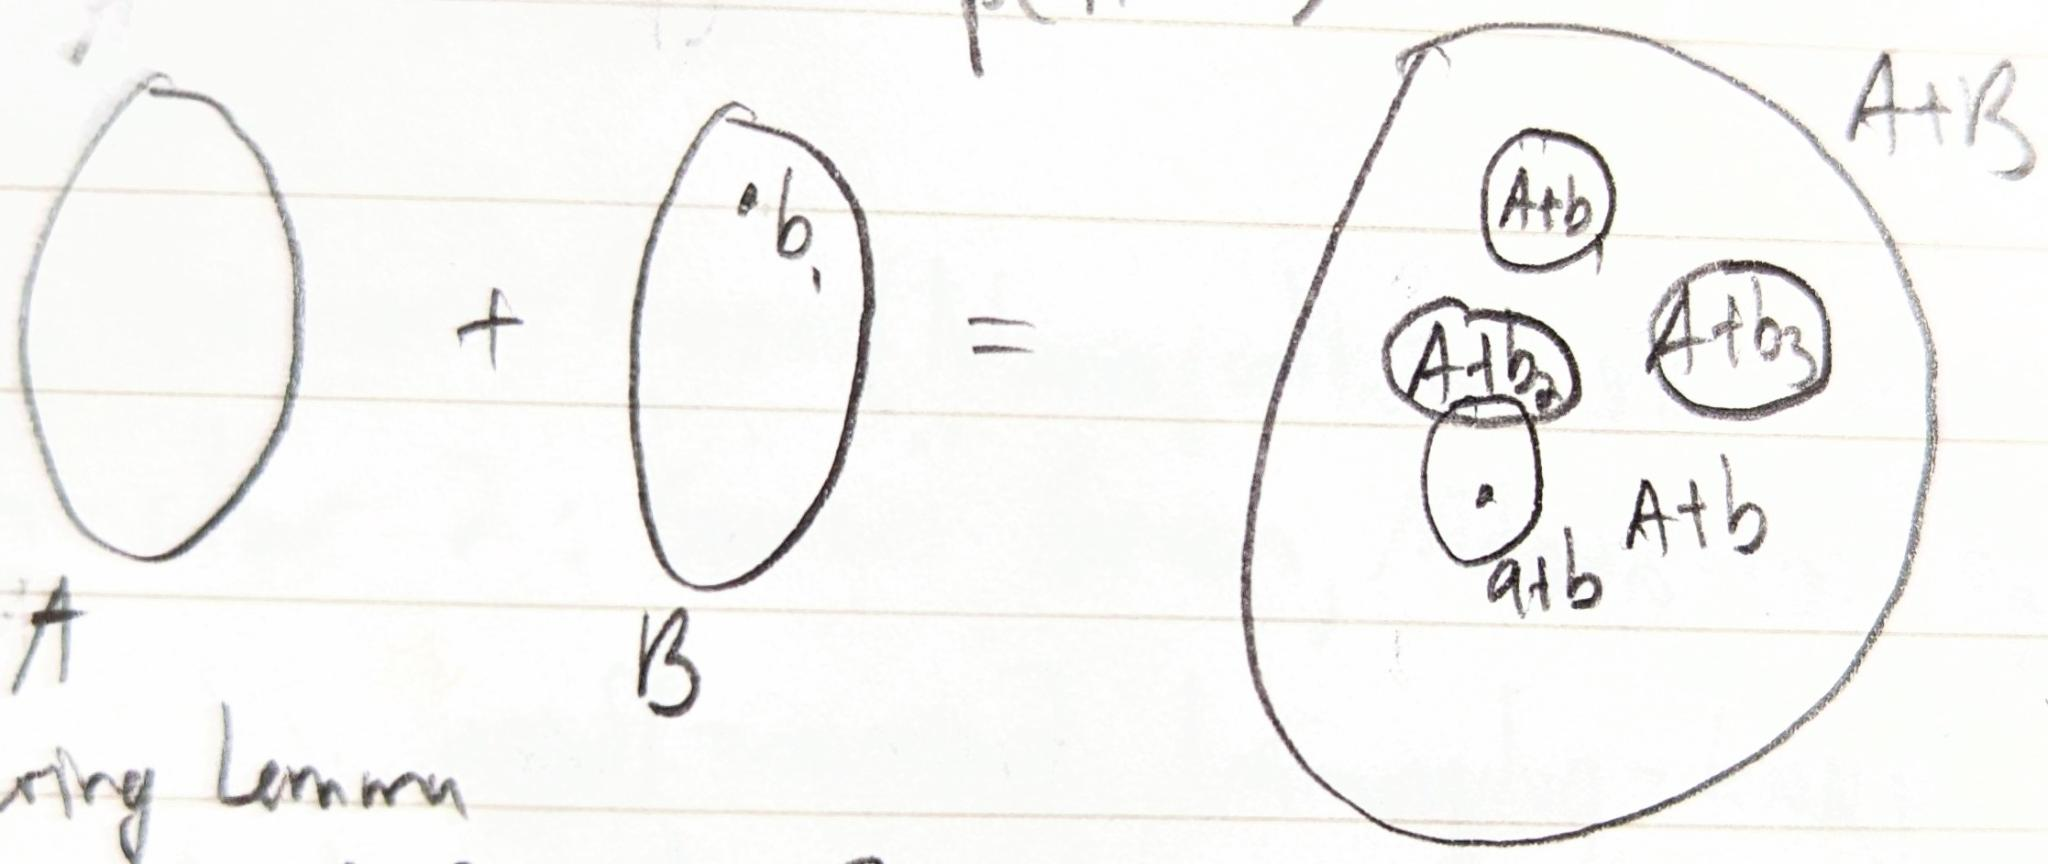
\includegraphics[width=.5\textwidth]{Rusza_covering}
	\caption{Rusza Covering Lemma \label{fig:Rusza_covering}}
\end{figure}

\begin{proof}
	1) is trivial.
	We are looking for the set $X = \{b_{1},\ldots, b_a\}$ that has the maximal number of translates that are pairwise disjoint.

	2) Fix an element $a+b \in A+ B $.
	Then $A + b $ has to intersect an element $x \in X $ s.t. $A+x \cap A+b \ne \emptyset $.
	Hence there is $a_{1} + b = a_{2} + x \iff b = a_{2}+x-a_{1} \implies \forall b \in B, \exists x \in X$ s.t. $b \in A - A + X$.
\end{proof}

\section{3/28/24}

Thus far we have been looking to cover $A $ with a GAP, and now we are covering a GAP with $2A-2A $.

First we prove Freiman:

\begin{proof}
	Let $A = P $ and $B = 2A-2A $ in the \Cref{lem:rusza_covering} $\rightarrow $ $X $ s.t. $|X| \le \frac{|P+2A-2A|}{||P|} $.
	Because $P\subseteq 2A-2A $,
	\[
		|X| \le \frac{|P+2A-2A|}{|P|} \le \frac{|4A-4A|}{|P|} \le \frac{|4A-4A|}{|A|}\exp(k^{O(1)}
	.\]

	Then $2A-2A \subseteq P -P + X $.
	WLOG, we can assume $0\in A $ (shift).
	Hence $A\subseteq 2A-2A \subseteq P - P +X $.

	So now all we need to do is to bound $\frac{|4A-4A|}{|A|} $.
	In the non-commutative case, this can be very large.
	In the torsion case, this can't be bounded, by letting $P = \Z_p $, which leads to $P-P $ being a gap, but may not be proper.
	To fix this, we introduce a new tool:
\end{proof}

\subsection{Properization}

\begin{thm}
	For any gap $P $ of rank $d $, there exists a proper gap of rank $d $ s.t. $P \subseteq Q $ and $|Q| \le |P|\cdot d^{O(d^3)}  $.
\end{thm}

Inuitively, $\rank(P) \le K^{O(1)}$, roughly $K $.

\subsection{Pl\"unecke-Rusza Inequalities}

\begin{thm}\label{thm:plunecke}
	$A,B \subseteq G $ s.t. $|A+B| = K |A| $.
	Then $|\pm B \pm B \pm B \pm \ldots \pm B |$ ($h $ times) $\le K^{h}|A|  $.
\end{thm}

\begin{cor}
	Suppose $B = A $.
	Then $k = \delta[A] $.
	The inequality then becomes
	\[
		|kA -\ell A| \le K^{k+\ell}|A|
	.\]
\end{cor}

The above Corollary then gives an upperbound on $\frac{|4A-4A|}{|A|} $, proving Freidman's Theorem.

Now let $\sigma[A] = \frac{|A-A|}{|A|} $.

\begin{cor}
	Then with $k = l = 1 $, $\sigma[A] \le \delta[A]^2$.
\end{cor}

Now this result is going to be very useful, especially in its generalized form for Gower's Theorem.

\begin{lem}[Rusza Triangle Inequality]
	Let $G $ be an ablian group.

	Combinatorial Form:
	\[
		|A-C| \le \frac{|A-B|\cdot |B-C|}{|B|}
	.\]
\end{lem}
\begin{proof}
	We WTS that $|B|\cdot |A-C| \le |A-B| \cdot |B-C| $.
	We prove it by finding an injective function $B\times (A-C) \rightarrowtail (A-B) \times (B-C) $

	$\forall x \in A - C $ (arbitrary but fixed), represent it as $x=a_x-c_x, a_x \in A, c_x \in C$.
	Then map
	\[
		(b,x) \mapsto (a_x-b,b-c_x)
	.\]
	Then say you're given $(a_x-b,b-c_x) $.
	Then you can recover a unique $x = a_x-b+b-c_x $ and from there recover $a_x,c_x $.
	This then gives $b $.
\end{proof}
\begin{lem}[Alternative Statement Rusza Triangle Inequality]
	\[
		\frac{|A-C|}{|A|^{\frac{1}{2}}|C|^{\frac{1}{2}} } \le \frac{|A-B|}{|A|^{\frac{1}{2}}|B|^{\frac{1}{2}}  } \cdot \frac{|B-C|}{|B|^{\frac{1}{2}}|C|^{\frac{1}{2}}  }
	.\]
\end{lem}

\begin{definition}[Rusza's Distance]
	\[
		\bm{d(A,C)} = \ln \frac{|A-C|}{|A|^{\frac{1}{2}}|C|^{\frac{1}{2}}  }
	.\]
\end{definition}

We can check that it is almost a metric (semimetric).
Since $|A-C| \ge \max(|A|,|C|) $, the fraction in the RHS is at least 1, showing that the RHS is non-negative.
Clearly it is symmetric.
By the Rusza Triangle Inequality, we have $d(A,C) \le d(A,B) + d(B,C) $.
But it violates positive definitiness (take $A,C $ part of the same subgroup).

From this we have that $d(A,-A) = \ln \delta[A] $ and that $d(A,A) = \ln \sigma [A] $.
Hence $\ln \sigma = d(A,A) \le d(A,-A) + d(A,-A) = 2\ln \delta [A] $

Now we return to the Pl\"unecke-Rusza Inequalities \ref{thm:plunecke}.

\begin{thm}
	With $K = \frac{|A+B|}{|A|}, |\pm B \pm B \pm \cdots \pm B| \le K^{h}|A|  $.
\end{thm}

Big Names: Petridis, Julia Walls, Jim Gowers

It began as a very complicated proof in 2016, but it was seriously streamlined.

\begin{proof}
	(Petridis')

	Consider a simple case:
	We prove that if $|A+B| \le K|A| $, then $|hB| \le K^h |A|$.

	If we decrease the RHS, then this inequality becomes stricter.
	So we can let $A $ be the smallest such set.
	Note that we have $B $ fixed the entire time.

	WLOG, $\forall A' \subset A, |A'+B| \ge K|A'| $.
	\begin{lem}
		Under all these assumptions, $|A+B+C| \le K|A+C| $ for an arbitrary $C $.
	\end{lem}

	This implies this case because $|hB| \le |A+hB| \le K|A+(h-1)B| \le K^2|A+(h-2)B| \le \cdots$ (let $C = (h-1)B $ in the lemma).
	This leads to $|hB| \le K^{h-1}|A+B| \le K^{h}|A|   $ (definition of $K $).

	\begin{proof}
		(Lemma)

		We do induction on $C $.
		Suppose it is true up to $|C| $ and we have $C' = C \cup \{x\}   $.
		Then $|A+B+C| \le K|A+C| $.
		We want $|A+B+C'| \le K|A+C'| $.

		We have $A+B+C' \subseteq (A+B+C)\cup (A+B+\{x\}), A+C' \subseteq (A+C) \cup (A+x)$ by definition.
		Suppose for a second that this (RHS) was a disjoint unions.
		Then because $|A+B+C| \le K|A+C|, |A+B+x| \le |A+x| $, completing the proof.

		By PIE (principle of inclusion exclusion), we have a $W $ s.t.
		\[
			W+x = (A+C)\cap (A+x)
		.\]
		This is a proper subset, because otherwise we are done (nothing else is added on both sides, i.e. $A+C' = (A+C)\cup(A+x) = A+x = A+C \implies |A+B+C'| \le |A+B+C|+|A+B+x| \le K|A+C| \le K|A+C'|$).
		So $W = (A+C-x) \cap A $.

		Next $(A+B+C)\cap(A+B+x) \supseteq W + x+B $ (we are supposing the LHS is small).
		By more PIE, we have that all we need to prove is that $|W+x+B| \ge K|W+x| $ and that $|W+B| \ge K|W|, W \subsetneq A $.

		Then double induction on $A $ and then top down.
	\end{proof}
\end{proof}

We are still focused on \Cref{lem:bogolubov-rusza}, i.e. that $\exists P\subseteq 2A-2A $ s.t. $|P| \ge |A| \exp(-K^{O(1)})  $.

The reason this is better than what we have before is that we can prove this for

\begin{enumerate}
	\item $A' \subseteq A, \frac{|A|}{|A'| \le \exp(K^{O(1)} }) ,$ \Cref{lem:bogolubov-rusza} for $A' \implies $ BR lemma for $A $
	\item BR Lemma is invariant under Freiman isomorphisms of order 8
\end{enumerate}

\begin{definition}
	Let $G,H $ be abelian groups, $A\subseteq G, B\subseteq H $.
	A \textbf{Freiman Homomorphism} of order $k $ is defined by
	\[
		(G,A) \xrightarrow{\phi} (H,B)
	\]
	s.t. $\phi:A\to B $ is a bijection between $A,B $ s.t.
	\[
		a_{1}+\ldots a_k = a_{1}'+\ldots a_k' \implies \phi(a_{1})+\ldots +\phi (a_k) = \phi (a_{1}') + \ldots +\phi (a_k').
	\]
\end{definition}

An example is an injective homomorphism that maps $a_{i} \mapsto a'_i $.
They are almost as good as homomorphisms, and they are indistinguishable up to $k $-tuples.

\begin{definition}
	A \textbf{Freiman isomorphism} is a Freiman homorphism whose inverse is a Freiman homomorphism.
\end{definition}

\begin{prop}
	If we have a Freiman isomorphism of order 8: $(G,A) \to (H,B) $, then BR lemma for $A $ is equivalent to BR lemma for $B $.
\end{prop}
\begin{proof}
	Clearly we have a Freiman homomorphism $(G,2A-2A) \to (H,2B-2B) $ of order 2.
	We have injectivity is because $\phi $ is bijective and well-defined.
	Now suppose we have a proper gap $P\subseteq 2A-2A $.
	Then $\phi(P) $ is a proper gap or subgroup of $H $.

	For $d=2 $, the gap is just a grid, and this grid is then translated into a wiggly grid.
	But we want it to be a full grid, and we have this by generating the right grid by the images of the terms on the LHS.

	We have the relation that $a_{1}+a_{4}=a_{2}+a_{3} \rightarrow b_{1}+b_{4}=b_{2}+b_{3}	$.
	As another example, $a_{1}+a_{5}=2a_{2} \rightarrow b_{1}+b_{5}=2b_{2} $.
	Simply repeat this.
	\begin{figure}[ht]
		\centering
		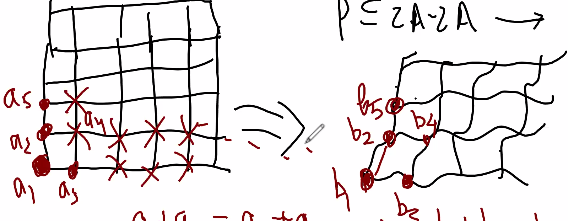
\includegraphics[width=.25\textwidth]{grid}
		\caption{Grid with $d=2 $ \label{fig:grid}}
	\end{figure}

	We will complete this proof on Tuesday.
\end{proof}

Next we will use basic Fourier analysis to reduce BR Lemma in $\Z $ to BR Lemma in $\Z_N $ where $N > 16|8A-8A| $.
By Chebyshev's theorem (?), we have $p\le K^{O(1)}  $ (also use Rusza Triangle inequality \ref{thm:plunecke-rusza}).

\begin{proof}
	We have $k=8 $ and $(\Z,A) \xrightarrow{k} (\Z_N,B) $.
	\begin{lem}
		$\exists A' \subseteq A $ with $|A'| \ge \frac{|A|}{k} $ and Freiman isomorphism between $(\Z,A')\xrightarrow{\phi}(\Z_N,B) $ where $N $ has the same restriction.
	\end{lem}
	\begin{proof}
		Outline of proof:
		The isomorphism is constructed with a huge $p $.
		We will find one
		\[
			(\Z,A') \xrightarrow{\phi} (\Z_p,L)\xrightarrow{\psi} (\Z_N,B)
		.\]
		THen $\phi $ is the quotient map, and $\psi $ is the remainder function.
		It takes $a\in \Z_p^{\times}  $, think about it as an integer, and $\psi(a) = a\pmod{N} $.
	\end{proof}
\end{proof}

\section{4/2/24}

The Freiman isomorphism definition is equivalent to
\begin{definition}
	A \textbf{Freiman isomorphism} of order $k $ is a map $\phi $ from $A\subseteq G $ to $B \subseteq H $ s.t.
	\[
		\phi(a_{1}) + \phi(a_{2}) + \cdots + \phi(a_k) = \phi(a_{1}') + \phi(a_{2}') + \cdots + \phi(a_k') \iff a_{1}+a_{2}+\cdots+a_k = a_{1}'+a_{2}'+\cdots+a_k'
	\]
	and $|A| = |B| $.
\end{definition}

We flesh out the proof of the lemma from before:
\begin{lem}
	$\forall A\subseteq \Z $ and $N \ge 2k|kA-kA|, \exists A'\subseteq A $ s.t. $|A'| \ge |A|/k $ and Freiman isomorphism $(\Z,A')\to (\Z,B) $ of order $k $ ($B \subseteq \Z_N $).
\end{lem}
\begin{proof}
	We construct the maps
	\[
		(\Z,A) \xrightarrow{\phi} (\Z_p,L) \to (\Z_n,B)
	\]
	with $p $ a sufficiently large prime.
	We find another $\phi_\lambda  $ s.t. it is also a Freiman isomorphism.
	Pick $\lambda \in \Z_p^{\times } $ (it remains flexible; random in a sense).
	Then we can let $\phi_\lambda \coloneqq  \lambda \circ \phi $ with $\phi $ being the quotient map $\Z\to \Z_p $.

	Split up $\Z_p $ into $k $ roughly equal intervals, where $\Z_p $ is represented by $\{0,1,\ldots ,p-1\}   $.
	Pick the interval containing the most points in $\lambda A $, call it $\lambda A' $.
	Then
	\[
		b_{1}+\cdots+b_k = b_{1}'+\cdots+b_k' \in \Z,\ b_i,b_i'\in \lambda A'
	\]
	iff
	\[
		b_{1}+\cdots+b_k \equiv b_{1}'+\cdots+b_k' \pmod{p}
	.\]
	Then we can translate this by intervals to extend $\lambda A' $ to a set of size $p $ with this property.

	Next let $\iota: \Z / N\Z \to \Z / p\Z $ (exists because $p $ is obscenely large).
	We WTS that
	\[
		\iota (b_{1})+\cdots+\iota (b_k) = \iota (b_{1}')+\iota (b_k') \pmod{N} \iff b_{1}+\cdots +b_k \equiv b_{1}'+\cdots +b_k' \pmod{N}
	.\]
	The only potential issue is if the LHS doesn't imply the RHS.
	Now consider the expression
	\[
		b_{1}+\cdots+b_k-b_{1}'-b_{2}'-\cdots-b_k' \pmod{N}
	.\]
	This is in $[-kp,kp] $ because $b_i,b_i' \in L $.
	Notice that there are $2kp / N $ ``bad'' intervals that are 0 mod $N $ and satisfy the iff in $\Z_p $.

	Finally, define
	\[
		\Delta \coloneqq  \{a_{1}+\cdots+a_k - a_{1}' - \cdots a_k' \ne 0 | a_i,a_i' \in A\}
	.\]
	Clearly $\Delta\subseteq \Z_p $ and $|\Delta| = |kA-kA| $.
	Consider $\lambda\Delta $.
	The $\lambda  $ we picked from before was flexible, so we can use a probabilitic argument to pick a lambda retroactively that avoids all the bad points.
	The probability that $\Delta $ has a bad point is $|\Delta|/p \cdot 2kp / N = |\Delta|\cdots 2k /N $, which is less than 1 by hypothesis.
\end{proof}

\subsection{Good Model (Dense)}

Let $k=8 $.
A good model gives us BR-Lemma in specific cases:

Our goal is to prove it true for $A\subseteq \Z_N $ ($\Z_2^N $) \footnote{I don't know what this means, but it was in my notes}.
It's dense because
\[
	|kA-kA| < K^{k}|A|, \mu = \frac{|A'|}{|G|}
.\]

Now we go on a tangent about the discrete Fourier transform.

\subsection{Discrete Fourier Analysis (on Abelian Groups)}

\subsubsection{Pontryagin Duality}

Fix a locally compact abelian group (topological group whose closure of neighborhoods are compact), e.g. $\Z $ is a discrete one.

\begin{definition}
\[
	\bm{T} = \R / \Z = \text{ the circle}
.\]
\end{definition}

\begin{definition}
	For a group $G $,
	\[
		\bm{\hat{G}} = \Hom(G,T) \text{ (continuous)}
	.\]
\end{definition}

\begin{thm}[Pontryagin Duality]
	\[
		\hat{\hat{G} } = G_i
	\]
	where $G_i$ is a separated component of $G $.
\end{thm}

\begin{example}
	$\hat{\Z} = T  $.
\end{example}

\begin{example}
	$\hat{T} = \Z  $ because $\exp(i\theta) \to \exp(i\alpha \theta ) $ are the morphisms, but not all $\alpha $ since $\exp $ has the periodic property.
	So we only want $\alpha = n \in \Z$.
\end{example}

\begin{definition}
 	Let $G $ be an abelian finite group.
	The \textbf{characters} of $G $ are elements of $\hat{G}  $, which are all group homomorphisms because we are using the discrete topology.
\end{definition}

For finite $G $, $\hat{G} = G  $, but this isn't canonical (depends on basis).
As such it isn't very useful.

To find $\hat{\Z_N}  $, we send $1\mapsto \xi_N $, and call this map $\chi(\xi) $.
In the particular case of $\Z_{2}^{N}  $, (fix standard basis of $e_{i} $), each $\chi_i: e_i \mapsto 1 $ or $-1 $.
So here, $S = \{i| \chi(e_i) = -1\}   $ implies that
\[
	\chi(S)(x_{1},\ldots,x_n) = (-1)^{\sum_{i\in S}x_i} = (-1)^{\left< x,S \right>}
.\]

To focus on discrete fourier transform, take an arbitrary $f: G\to \C $.

\begin{definition}
	\[
		\bm{\left< f,g \right>} = \mathbb{E}_{x\in_R G}[f(x)\overline{g}(x)]
	.\]
	with $\mathbb{E} $ the expectation.\footnote{I don't know what the subscript in expectation means}
\end{definition}

The conjugation is needed for it to be a Hermitian inner product.

\begin{definition}
	The discrete Fourier transform is
	\[
		\hat{f}:\hat{G} \to \C
	\]
	s.t. $\hat{f}(\chi) = \left< f,\chi  \right>  $.
\end{definition}

\begin{property}
	\begin{enumerate}
		\item $\left< \chi ,\chi  \right> =1$
		\item Orthogenality property: for $\chi_{1}(x_{0})\ne \chi_{2}(x_{0} $ for some $x_{0} $,
			\[
				\left< \chi_{1},\chi_{2} \right> = 0
			.\]
	\end{enumerate}
\end{property}
\begin{proof}
	1) Obvious

	2) Note that conjugation of characters is inversion.
	\[
		\mathbb{E}_x[\chi_{1}(x)\chi_{2}^{-1}(x)] = \mathbb{E}_x[\chi_{1}(x+x_{0})\chi_{2}^{-1}(x+x_{0})] = \chi_{1}(x_{0})\chi_{2}(x_{0})^{-1}\mathbb{E}[\chi_{1}(x)\chi_{2}^{-1}(x)]
	.\]
	Hence $\chi_{1}(x_{0}) \chi_{2}(x_{0})^{-1} \ne 1 \implies \left< \chi_{1},\chi_{2} \right> = 0$.
\end{proof}

Look at a $G\times \hat{G}  $ matrix.
It is unitary because of the above properties.
\[
	\begin{pmatrix} \chi_{1} & \chi_{2} & \cdots \end{pmatrix}  \implies |\hat{G}| = |G|
.\]
The Hadamard matrix is another name for matrix.

Then
\[
	f(x) = \sum_{\chi \in \hat{G} } \hat{f}(\chi)\chi(x)
.\]

\begin{exercise}
	We might want conjugation.
\end{exercise}

When you translate back and forth, you lose a factor of $\frac{1}{N^{\frac{1}{2}} } $, but not here because we don't care and it's built into expectation.

\begin{thm}[Parseval's Identity]
	\[
		|f|^2 = \mathbb{E}_x[|f(x)|^2] = \sum_{\chi} |\hat{f}(\chi )|^2
	.\]
\end{thm}

\subsubsection{Convolution}

\begin{definition}
	\[
		\bm{(f\ast g)(x)} \coloneqq \mathbb{E}_y[f(x-y)g(y)] = \mathbb{E}_{y_{1},y_{2}}[f(y_{1})g(y_{2})|y_{1}+y_{2}=x]
	.\]
\end{definition}

$f,g $ give probability distributions over $G $, and the convolution is basically interpolating them and making it nicer.

\begin{prop}
	\[
		\hat{f\ast g} = \hat{f}\cdot \hat{g}
	.\]
\end{prop}
\begin{proof}
	We WTS that $\widehat{f\ast g} = \hat{f}\hat{g}    $.
	We only need to show that $\forall x\in \hat{G}  $ we have $\left< f\ast g,x \right> = \left< f,x \right>\left< g,x \right> $.

	We have that
	\[
		\left< f\ast g,x \right> = \mathbb{E}_{x,y}[f(x-y)g(y)\chi ^{-1}(x)]
	.\]
	Then letting $z = x-y $ gives
	\[
		\mathbb{E}_{y,z}[f(z)g(y)\chi ^{-1}(y+z)] = \mathbb{E}_{y,z}[f(z)g(y)\chi ^{-1}(y)\chi (z)]
	.\]
	This then equals
	\[
		\left< f,x \right>\left< g,x \right>
	.\]
\end{proof}

We mostly care about \footnote{the below may be wrong}
\begin{definition}
\[
	\bm{\mathbb{L}_A} =
	\begin{cases}
		1 & x\in A\\
		0 & \text{ else}
	\end{cases}
.\]
\footnote{I can't tell what the symbol here is, I assume it's a bold font L}
\end{definition}

\begin{thm}
	\[
		|\mathbb{L}_A|^2 = \mu = \sum_{\chi} |\chi(\mathbb{L})|^2
	.\]
\end{thm}

\begin{lem}
	\[
		|\chi(\mathbb{L}_A)|^4 \ge \mu^4
	.\]
\end{lem}
\begin{proof}
	Consider $\widehat{\mathbb{L}_A\ast \mathbb{L}_{A}\ast \mathbb{L}_{-A}\ast\mathbb{L}_{-A}} = \hat{\mathbb{L}_A}\ast \hat{\mathbb{L}_A}\ast \hat{\mathbb{L}_{-A}}\ast \hat{\mathbb{L}_{-A}} = |\mathbb{L}_A|^{4} $.
\end{proof}
\end{document}
